\chapter{Programmable Hinge Mechanics for Functional Reconfigurable Trusses}\label{chapter-04}


\section{Introduction}\label{04-sec-functional-intro}
The remainder of the chapter is organized as follows. Section~\ref{04-sec-bounded-rotation} introduces an enhanced formulation of the torsional spring that limits its deformation range and enables study of sequential folding of kinematic degrees of freedom of the reconfigurable truss. Next, Section~\ref{04-sec-multistable-hinge} introduces a multistable torsional hinge design which employs magnetic interaction to achieve multiple stable states. This section also develops a computational model of the magnetic multistable hinge building on the 3NTS model. Section~\ref{04-sec-bistable-spring} introduces a way to model bistable behavior into the 3NTS element and demonstrates reconfigurable trusses with more than one degree of freedom exhibit multiple stable states based on 2 stable states per kinematic degree of freedom. Section~\ref{04-sec-discussion} presents a discussion on the possible applications of the analysis tools and the potential applications the nonlinear hinge modeling enables. Finally, the concluding remarks are presented in Seciton~\ref{04-sec-conclusion}.

\section{Modeling Bounded Rotation in Torsional Spring Hinges}\label{04-sec-bounded-rotation}
This section builds on the Three-Node Torsional Spring (3NTS) element from Chapter~\ref{chapter-03} to enforce limits on the angular rotation of the joints. The enhanced constitutive law preserves the linear spring response within the intended operating range and introduces nonlinear stiffening near the deformation limits. This bounded response prevents inadmissible hinge rotations and enables the analysis of sequential folding, locking, and load redistribution in reconfigurable trusses.

\subsection{Enhanced Torsional Spring Constitutive Law}\label{04-subsec-enhanced-spring}
The Three-Node Torsional Spring (3NTS) element was originally formulated using a linear torsional spring constitutive law. In this formulation, the spring deformation is described by the relative angle \(\alpha\) defined over the interval \([0,~2\pi)\). The spring's restoring moment is proportional to the difference between the current relative angle \(\alpha\) and the rest angle \(\alpha_0\). While this formulation works as long as \(0 \le \alpha < 2\pi\), numerical issues arise when the spring undergoes large rotations associated with self-overlap of the connected bars. Since \(\alpha\) is evaluated over [\(0,~2\pi\)), the computed angle wraps from \(2\pi\) to 0 when the rotation exceeds this range. This behavior produces a sudden discontinuity in the computed spring deformation, leading to inconsistent restoring moments and tangent stiffness with the actual deformation path.

This numerical issue is also inconsistent with the observed physical behavior of the reconfigurable truss systems discussed in this dissertation. In these systems, the bars connected to a torsional spring do not overlap each other during reconfiguration. The fabrication techniques and kinematics of the truss physically limit the allowable rotation at each folding joint, as discussed in Chapter~\ref{chapter-02} (see Fig.~\ref{fig-warren-test}\,(c)). Furthermore, relative angles near 0 or \(2\pi\) correspond to a fully actuated degree of freedom, where the truss has reached its most compact configuration. Rotation of the spring joint beyond this state becomes meaningless. Therefore, rotations beyond 0 or \(2\pi\) do not represent the intended deformation range of the torsional springs in the physical structure. This motivates restricting the admissible angular range of the torsional spring.

To address the numerical issue and ensure that the spring model captures a realistic range of deformation for the folding joints, the constitutive law of the 3NTS element is modified using the concepts inspired by the bar-and-hinge model~\cite{liu2017merlin}. The modified formulation restricts the admissible deformation range of the spring by introducing nonlinear stiffening near the extreme deformation limits. This stiffening acts as a smooth mechanical stop, providing increasing resistance as the joint approaches its allowable rotation limit. The modified formulation, referred to as the \textit{Enhanced Spring Law}, preserves the original linear response near the rest configuration while creating high-energy barriers at the lower and upper deformation limits.

The enhanced spring law introduces three additional parameters to define the admissible deformation limits of the spring. The parameter, \(\delta\), defines the minimum allowable relative angle between the two connected members. Therefore, the lower admissible deformation limit of the spring becomes \(\delta\). By symmetry, the upper admissible limit becomes \(2\pi-\delta\). The parameters \(\alpha_1\) and \(\alpha_2\) define the lower and upper threshold angles, respectively, at which the spring response transitions from the linear to the nonlinear stiffening regime. These parameters satisfy the following relationship: \(0 \le \delta < \alpha_1 < \alpha_0 < \alpha_2 < 2\pi-\delta \le 2\pi\). Thus, the interval [\(\alpha_1,~\alpha_2\)] represents the nominal operating range of the spring. Within this range, the enhanced law is identical to the original linear torsional spring law. The intervals (\(\delta,~\alpha_1\)) and (\(\alpha_2,~2\pi-\delta\)), on the other hand, represent the nonlinear stiffening regions near the lower and upper deformation limits, respectively.

\begin{figure}[!ht]
  \centering
  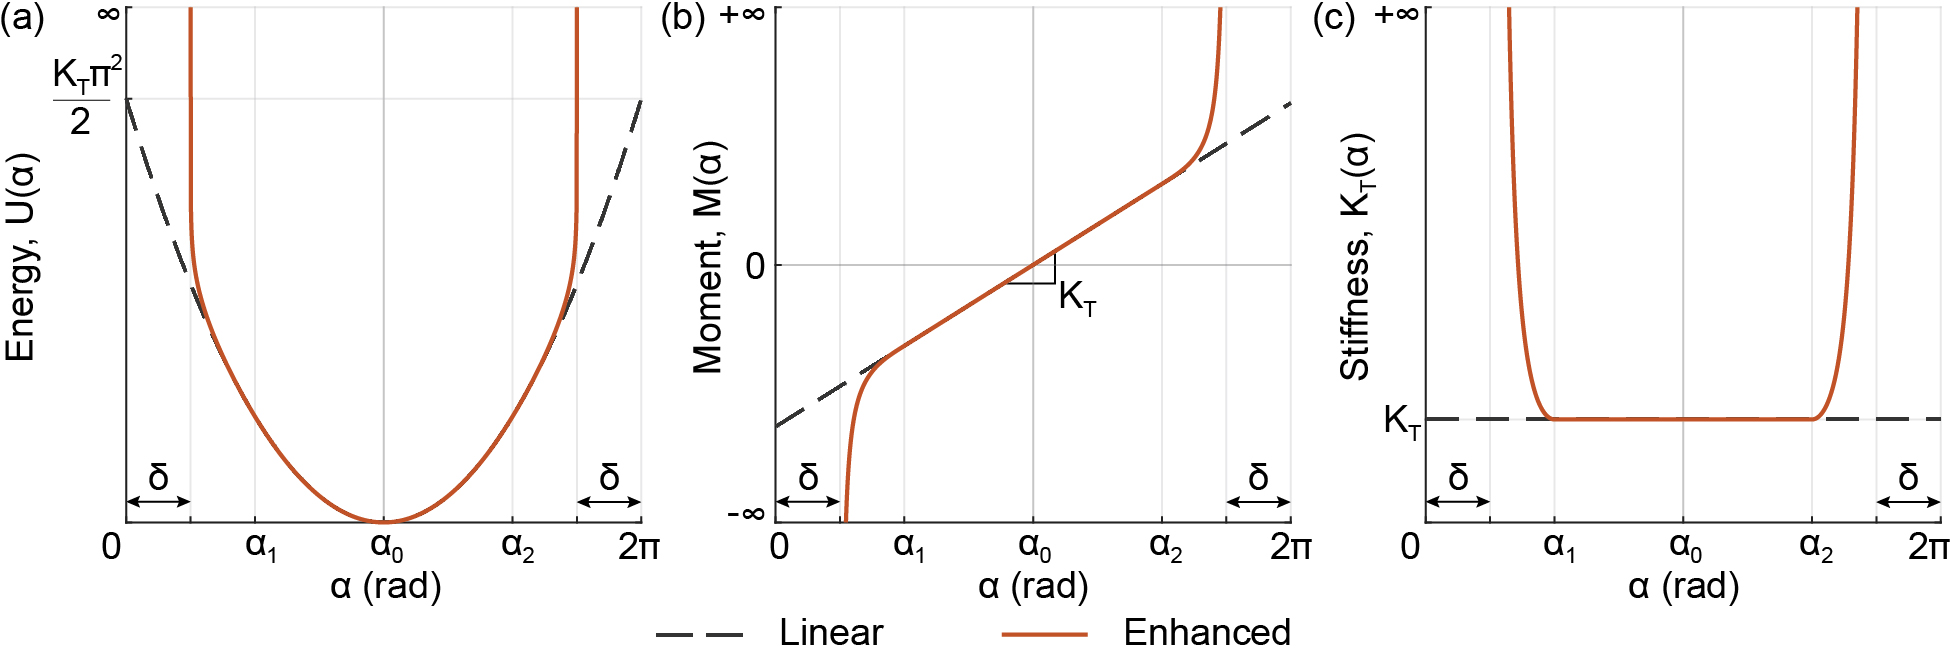
\includegraphics[width=\textwidth]{01-figures/04-01-spring-law-comparison.jpg}
  \caption{Comparison between the original linear torsional spring law (dashed line) and the enhanced spring law (solid line): (a) strain energy; (b) restoring moment; and (c) tangent stiffness as functions of the relative angle \(\alpha\). Here, \(\alpha_0\) is the rest angle, \(\alpha_1\) and \(\alpha_2\) are the lower and upper threshold angles where the spring response changes from linear to nonlinear stiffening, respectively, and \(\delta\) and \(2\pi-\delta\) are the lower and upper admissible deformation limits, respectively.}\label{fig-spring-law-comparison}
\end{figure}

The strain energy, U(\(\alpha\)), of the enhanced spring law is defined as
\begin{flalign}
\quad{}U(\alpha)&=
\begin{cases}
\frac12 K_T(\alpha_0-\alpha_1)^2
+ K_T(\alpha_0-\alpha_1)(\alpha_1-\alpha)
\\- \frac{4K_T(\alpha_1-\delta)^2}{\pi^2}
\ln\!\left|\cos\!\left(\frac{\pi(\alpha_1-\alpha)}{2(\alpha_1-\delta)}\right)\right|, & \alpha < \alpha_1 \\[24pt]
\frac12 K_T(\alpha-\alpha_0)^2, & \alpha_1 \le \alpha \le \alpha_2 \\[24pt]
\frac12 K_T(\alpha_2-\alpha_0)^2
+ K_T(\alpha_2-\alpha_0)(\alpha-\alpha_2)
\\- \frac{4K_T((2\pi-\delta)-\alpha_2)^2}{\pi^2}
\ln\!\left|\cos\!\left(\frac{\pi(\alpha-\alpha_2)}{2((2\pi-\delta)-\alpha_2)}\right)\right|, & \alpha > \alpha_2
\end{cases}&\label{eq-enhanced-energy}
\end{flalign}

The restoring moment of the enhanced spring is obtained as the first derivative of the strain energy with respect to the relative angle \(\alpha\) as
\begin{flalign}
\quad{}M(\alpha)&=
\begin{cases}
K_T(\alpha_1-\alpha_0) + \dfrac{2K_T(\alpha_1-\delta)}{\pi}\tan\Bigg(\frac{\pi(\alpha-\alpha_1)}{2(\alpha_1-\delta)}\Bigg),
& \alpha < \alpha_1 \\[24pt]
K_T(\alpha-\alpha_0),
& \alpha_1 \le \alpha \le \alpha_2 \\[24pt]
K_T(\alpha_2-\alpha_0) + \dfrac{2K_T(2\pi-\delta-\alpha_2)}{\pi}\tan\Bigg(\frac{\pi(\alpha-\alpha_2)}{2(2\pi-\delta-\alpha_2)}\Bigg),
& \alpha > \alpha_2
\end{cases}&\label{eq-enhanced-moment}
\end{flalign}

The corresponding tangent rotational stiffness of the enhanced spring is obtained as the derivative of the restoring moment with respect to \(\alpha\) as
\begin{flalign}
\quad{}K_T(\alpha)&=
\begin{cases}
K_T\,\sec^2\Bigg(\frac{\pi(\alpha-\alpha_1)}{2(\alpha_1-\delta)}\Bigg), & \alpha < \alpha_1\\[24pt]
K_T,& \alpha_1 \le \alpha \le \alpha_2
\\[24pt]
K_T\,\sec^2\Bigg(\frac{\pi(\alpha-\alpha_2)}{2((2\pi-\delta)-\alpha_2)}\Bigg), & \alpha > \alpha_2
\end{cases} & \label{eq-enhanced-stiffness}
\end{flalign}

Figure~\ref{fig-spring-law-comparison}\,(a-c) compares the original linear torsional spring law (dashed line) with the enhanced spring law (solid line) in terms of strain energy, restoring moment, and tangent rotational stiffness. It is important to note that the values of \(\delta\), \(\alpha_1\), and \(\alpha_2\) used in Fig.~\ref{fig-spring-law-comparison} are chosen for visual representation only and are not up to scale. 

The spring response can be divided into three regions. Firstly, when \(\alpha_1 \le \alpha \le \alpha_2\), the enhanced law reduces to the original 3NTS constitutive law. The tangent stiffness is constant and equal to \(K_\textrm{T}\), the restoring moment varies linearly with \(\alpha-\alpha_0\), and the strain energy varies quadratically with \(\alpha-\alpha_0\). The energy minimum occurs at \(\alpha=\alpha_0\), where the restoring moment is zero. Thus, the enhanced law does not alter the spring response in the intended operating range. In the lower stiffening region, where \(\delta < \alpha < \alpha_1\), the spring stiffens as the relative angle decreases below \(\alpha_1\). The tangent stiffness increases according to a secant-squared function and tends to infinity as \(\alpha \rightarrow \delta^+\). The restoring moment becomes increasingly negative. This moment resists further closure of the joint. The strain energy also grows rapidly as the lower admissible limit is approached. In the upper stiffening region, where \(\alpha_2 < \alpha < 2\pi-\delta\), the spring stiffens as the relative angle increases beyond \(\alpha_2\). The tangent stiffness again tends to infinity, now as \(\alpha \rightarrow (2\pi-\delta)^-\). The restoring moment becomes increasingly positive. This moment resists further deformation of the joint. The strain energy also grows rapidly near the upper admissible limit.

\subsection{Path-dependent loading and Sequential Folding Enabled by Enhanced Torsional Spring}\label{04-subsec-deployment-path}

The enhanced spring law formulated in the previous subsection allows the 3NTS element to model large rotations while enforcing prescribed angular limits. This capability is important for reconfigurable trusses with multiple independent kinematic degrees of freedom. In such systems, individual units may fold, lock, or remain active at different stages of deformation. The enhanced spring law allows the simulation of these transitions without numerical failure caused by angle wrapping, spring overlap, or physically inadmissible rotations. This subsection demonstrates these capabilities using two examples.

The first example is the stacked square-linkage truss shown in Fig.~\ref{fig-deployment-path}\,(a). The structure consists of two vertically stacked square units. Each unit is a special case of a six-bar linkage, formed by a square frame and two diagonal bars with a rotational joint at their connection. The joint at the midpoint of each diagonal is modeled using the enhanced torsional spring. Each unit, therefore, contributes one independent kinematic degree of freedom to the structure.

The structure is approximately 2~m tall. Each non-diagonal member has a length of 1~m. The bars have an elastic modulus \(E = 3\times10^9~\text{Pa}\) and a cross-sectional area \(A = 0.5~\text{m}^2\). Each torsional spring has a linear-regime stiffness \(K_T = 10~\text{Nm/rad}\). A geometric imperfection of \(10^\circ\) is assigned to each torsional spring joint to simulate buckling deformation of the diagonal bars. The admissible rotation range is bounded between \(15^\circ\) and \(345^\circ\) and the spring response remains linear between \(30^\circ\) and \(330^\circ\). Outside this interval, the tangent stiffness increases asymptotically as the spring angle approaches the prescribed maximum angular deformation limits. Using the notation from the previous subsection, these enhanced spring law parameters are set to \(\alpha_1 = 30^\circ\), \(\alpha_2 = 330^\circ\), and \(\delta_1 = 15^\circ\).

The load-displacement response of the stacked square-linkage truss is shown in Fig.~\ref{fig-deployment-path}\,(b). At the beginning of loading, both units resist the applied vertical load. The structure carries a load of approximately 180~N before instability develops in the lower unit. After this instability, the load drops as the lower unit folds. The lower unit continues to deform until the relative angle of its torsional spring approaches the lower angular limit of \(15^\circ\). At this stage, the enhanced spring law makes the torsional spring increasingly stiff, preventing any further deformation of the lower unit.

After the lower unit locks, additional load on the system is redistributed and transferred to the upper unit. The load then increases again, leading to a second instability in the upper unit. The upper unit folds like the lower unit until its torsional spring also approaches the lower angular limit. Once both the units are locked, any further increase of load on the structure is resisted by a combination of the axial deformation of the bars and the extremely stiff torsional springs. This produces the final steep increase in the load-displacement curve near \(\Delta = 1.6~\text{m}\), as shown in Fig.~\ref{fig-deployment-path}\,(b).

\begin{figure}[!ht]
  \centering
  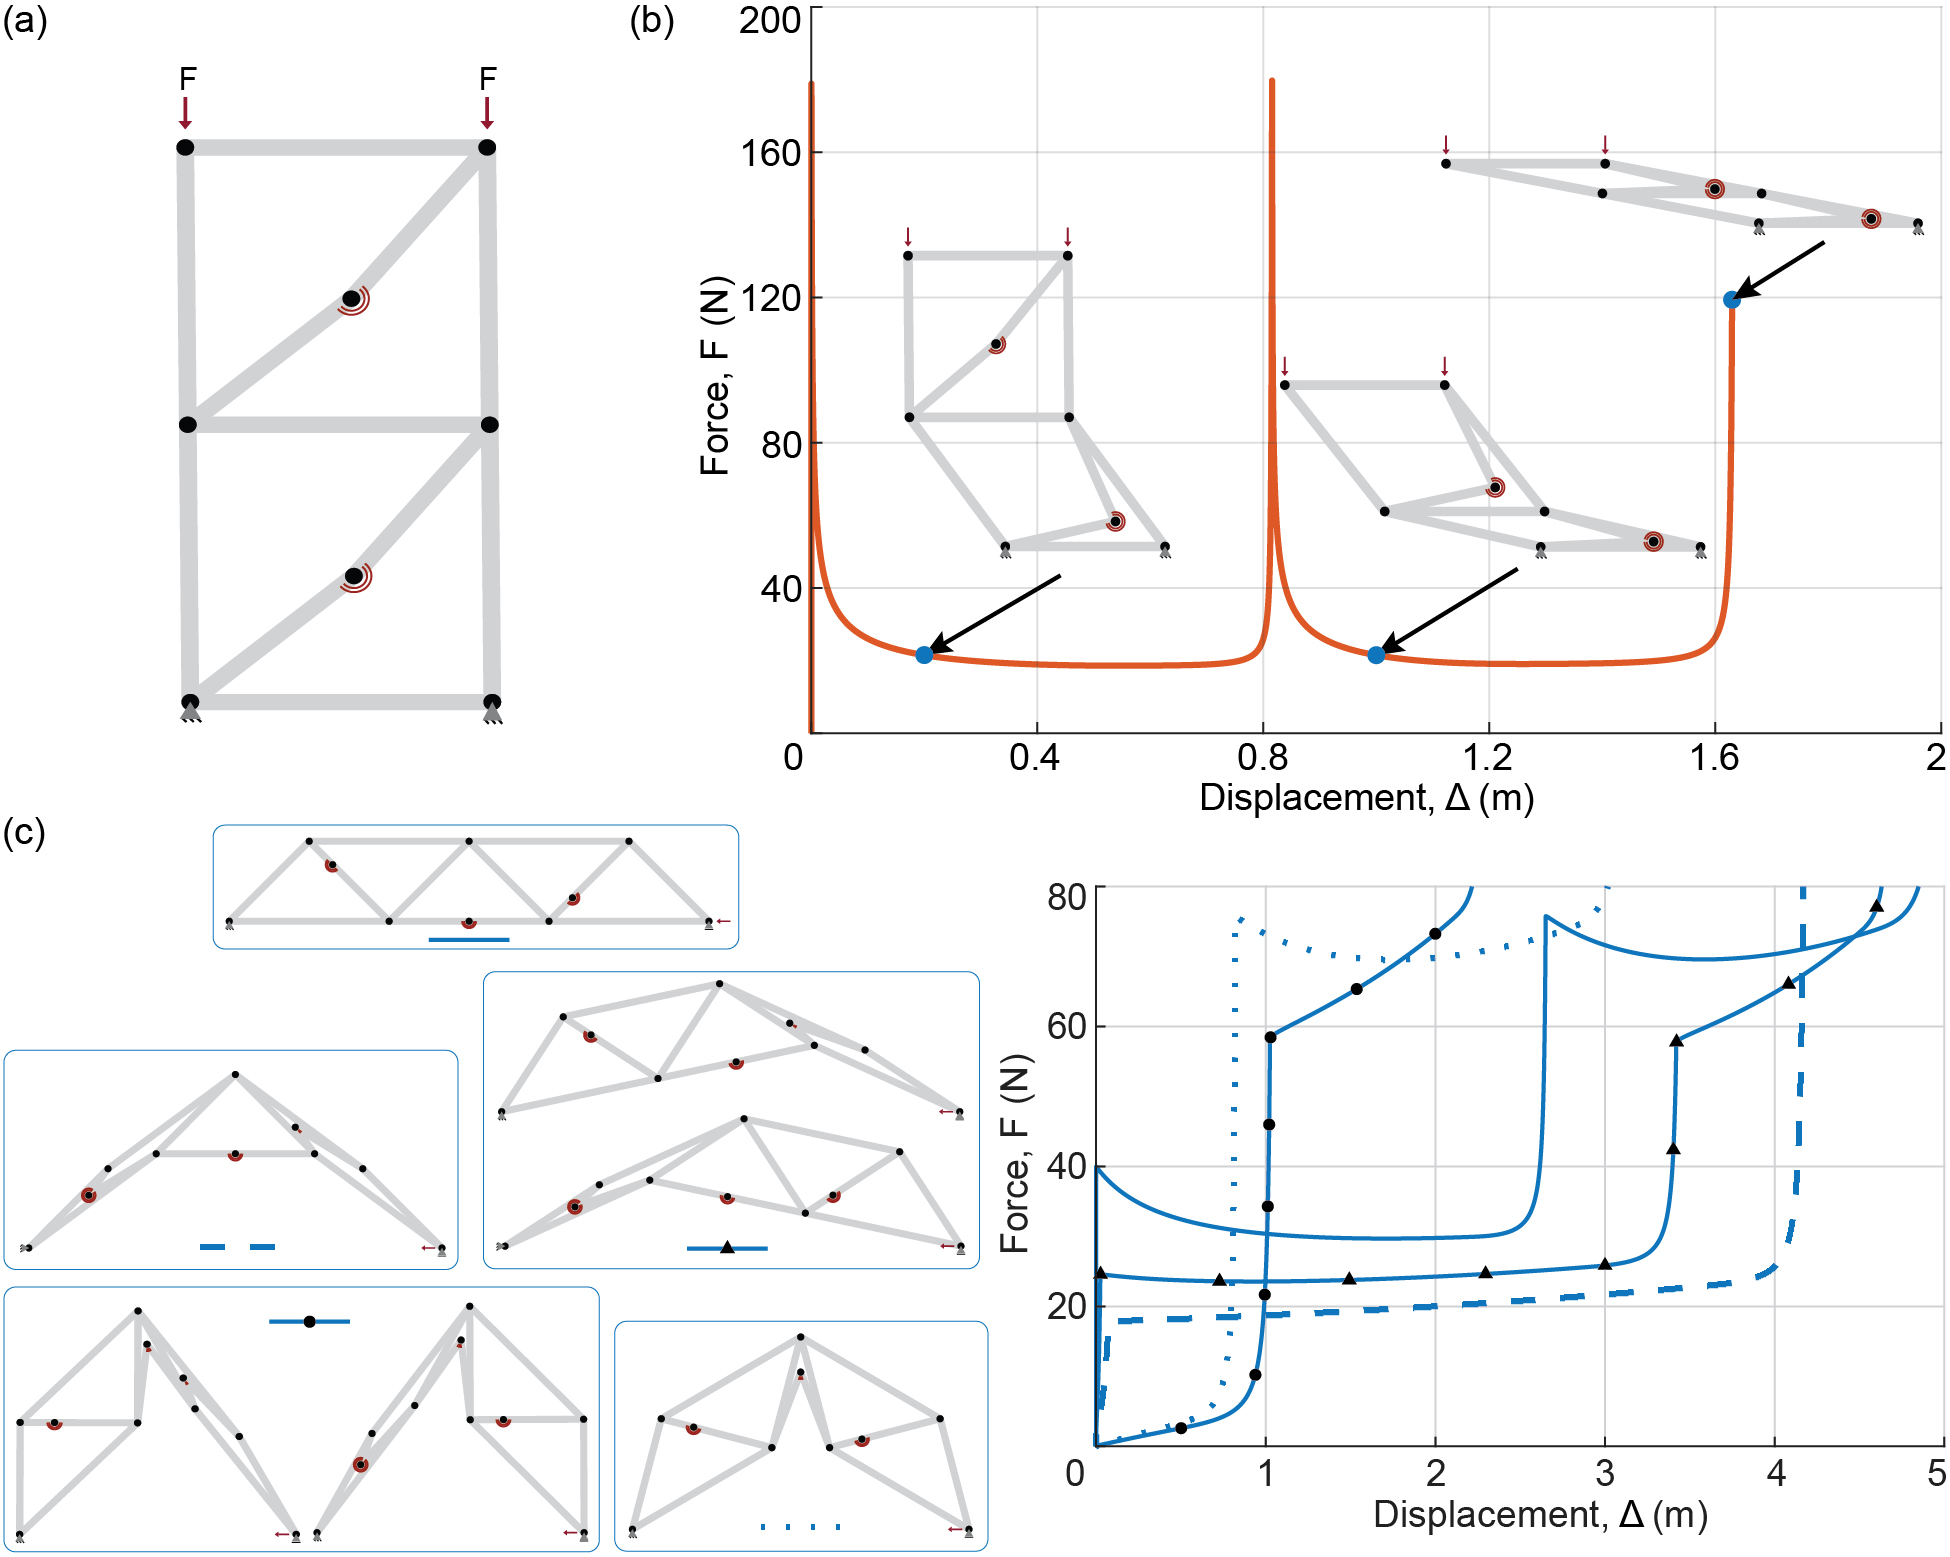
\includegraphics[width=\textwidth]{01-figures/04-02-path-analysis.jpg}
  \caption{(a) Vertically stacked square-linkage truss with two independent folding units under compression. Each unit contains an enhanced torsional spring at the midpoint of the diagonal member; (b) Load-displacement response showing sequential development of instability, folding, and locking of the structure's kinematic units; (c) Reconfigurable Warren truss configurations produced by folding different combinations of its independent kinematic units; (d) Load-displacement responses for folding various Warren truss configurations to the same compact state. The intermediate force demand depends on the folding path, even when the maximum force required to fold the entire structure is the same.}\label{fig-deployment-path}
\end{figure}

This example illustrates the main advantage of the enhanced spring law. The formulation can capture sequential folding, locking, and load redistribution in a reconfigurable truss with multiple independent kinematic degrees of freedom. A conventional linear torsional spring cannot represent this behavior reliably because it does not impose a physical angular range. The enhanced law therefore provides a way to study collapse sequences, deployment sequences, and actuation paths in systems in which different units activate at different stages of deformation.

The second example considers the reconfigurable Warren truss and its various configurations shown in Fig.~\ref{fig-deployment-path}\,(c). The truss is 6~m long and 1~m high. The left support is pinned, and the right support is modeled as a roller. Three enhanced torsional springs are placed at the locations marked with red arcs, as shown in Fig.~\ref{fig-deployment-path}\,(c). Since the structure has three independent kinematic degrees of freedom, the structure can occupy several intermediate configurations depending on which units remain folded or open. Excluding symmetric cases, the truss has five unique starting configurations shown in Fig.~\ref{fig-deployment-path}\,(c).

Each configuration is loaded by applying a vertical displacement at the roller support in the negative y-direction. The corresponding load-displacement curves are shown in Fig.~\ref{fig-deployment-path}\,(d). Each torsional spring has a geometric imperfection of \(0.1^\circ\), and the linear-regime torsional stiffness is set at \(K_T = 20~\text{Nm/rad}\).

The results show that all loading paths eventually require approximately 80~N to reach the most compact final state. However, the force demand varies substantially during the intermediate stages of folding. This variation occurs because each starting configuration activates a different set of kinematic degrees of freedom. Some configurations deform through a gradual folding sequence. Others require one or more units to snap through or lock before the remaining units can continue to fold. As individual units reach their angular limits, the enhanced springs restrict further rotation and redirect deformation to the remaining active units.

Therefore, the final compact configuration alone does not define the actuation demand. The required force also depends on the folding path used to reach that configuration. The enhanced torsional spring law makes this path dependence accessible in simulation. It allows the force demand to be evaluated for different deployment or collapse sequences while maintaining physically admissible joint rotations. This capability is useful for designing reconfigurable trusses that must fold in a prescribed order, avoid unintended locking, or minimize actuation forces along a selected kinematic path.

\section{Magnetic Multi-stable Torsional Hinges}\label{04-sec-multistable-hinge}
This section presents a magnetic multistable torsional hinge that uses polarity-dependent interactions between permanent magnets to create multiple stable rotational states. The physical design, fabrication, and reduced-order torque--rotation model are first introduced to characterize the hinge behavior. The multistable hinge response is then incorporated into the 3NTS element formulation, enabling programmable mechanical response in the reconfigurable trusses.

\subsection{Prototype and Reduced-order Simulated Response of a Magnetic Multistable Hinge}\label{04-subsec-magnetic-hinge-prototype}
The magnetic torsional hinge prototype uses polarity-dependent interactions between permanent magnets to create preferred rotational states. The hinge is formed at the joint between two axial members whose ends remain adjacent during rotation. Each member terminates in a circular hub, which provides the mating surface for the magnetic connection, as shown in Fig.~\ref{fig-magnetic-prototype}\,(a). Each hub face contains eight identical N35-grade cylindrical neodymium magnets with a diameter of 6~mm and a thickness of 2~mm. The magnets are seated in individual holes and are equally spaced at 45\(^\circ{}\) intervals around the hinge axis. The center of each magnet lies on a pitch circle with a radius of 13.75~mm. The opposing hub uses the same geometric layout, so corresponding magnets align face-to-face when the two hubs are in selected relative orientations. The exposed poles alternate between north and south around each hub face, and the pole sequence on the opposing hub is arranged so that aligned magnet pairs have opposite-facing poles in the preferred configurations. As the hubs rotate relative to each other, the facing magnet pairs move between attractive and repulsive alignments, producing a periodic magnetic torque and multiple stable rotational states. The hub dimensions and magnet layout are shown in Fig.~\ref{fig-magnetic-prototype}\,(a).

As one hub rotates relative to the other, the facing magnet pairs periodically move between attracting and repelling configurations. Stable states occur at relative rotations where the two magnet arrays form an energetically favorable pole arrangement. For the eight-magnet alternating-polarity pattern used in this prototype, the magnetic layout repeats every \(\pi/2\) radians, resulting in four stable states over one full rotation. Figure~\ref{fig-magnetic-prototype}\,(b, left) shows the 3D-printed hinge components with embedded magnets, and Fig.~\ref{fig-magnetic-prototype}\,(b, right) shows the four stable configurations of the magnetic multistable hinge integrated into a four-bar linkage unit.

\begin{figure}[!ht]
  \centering
  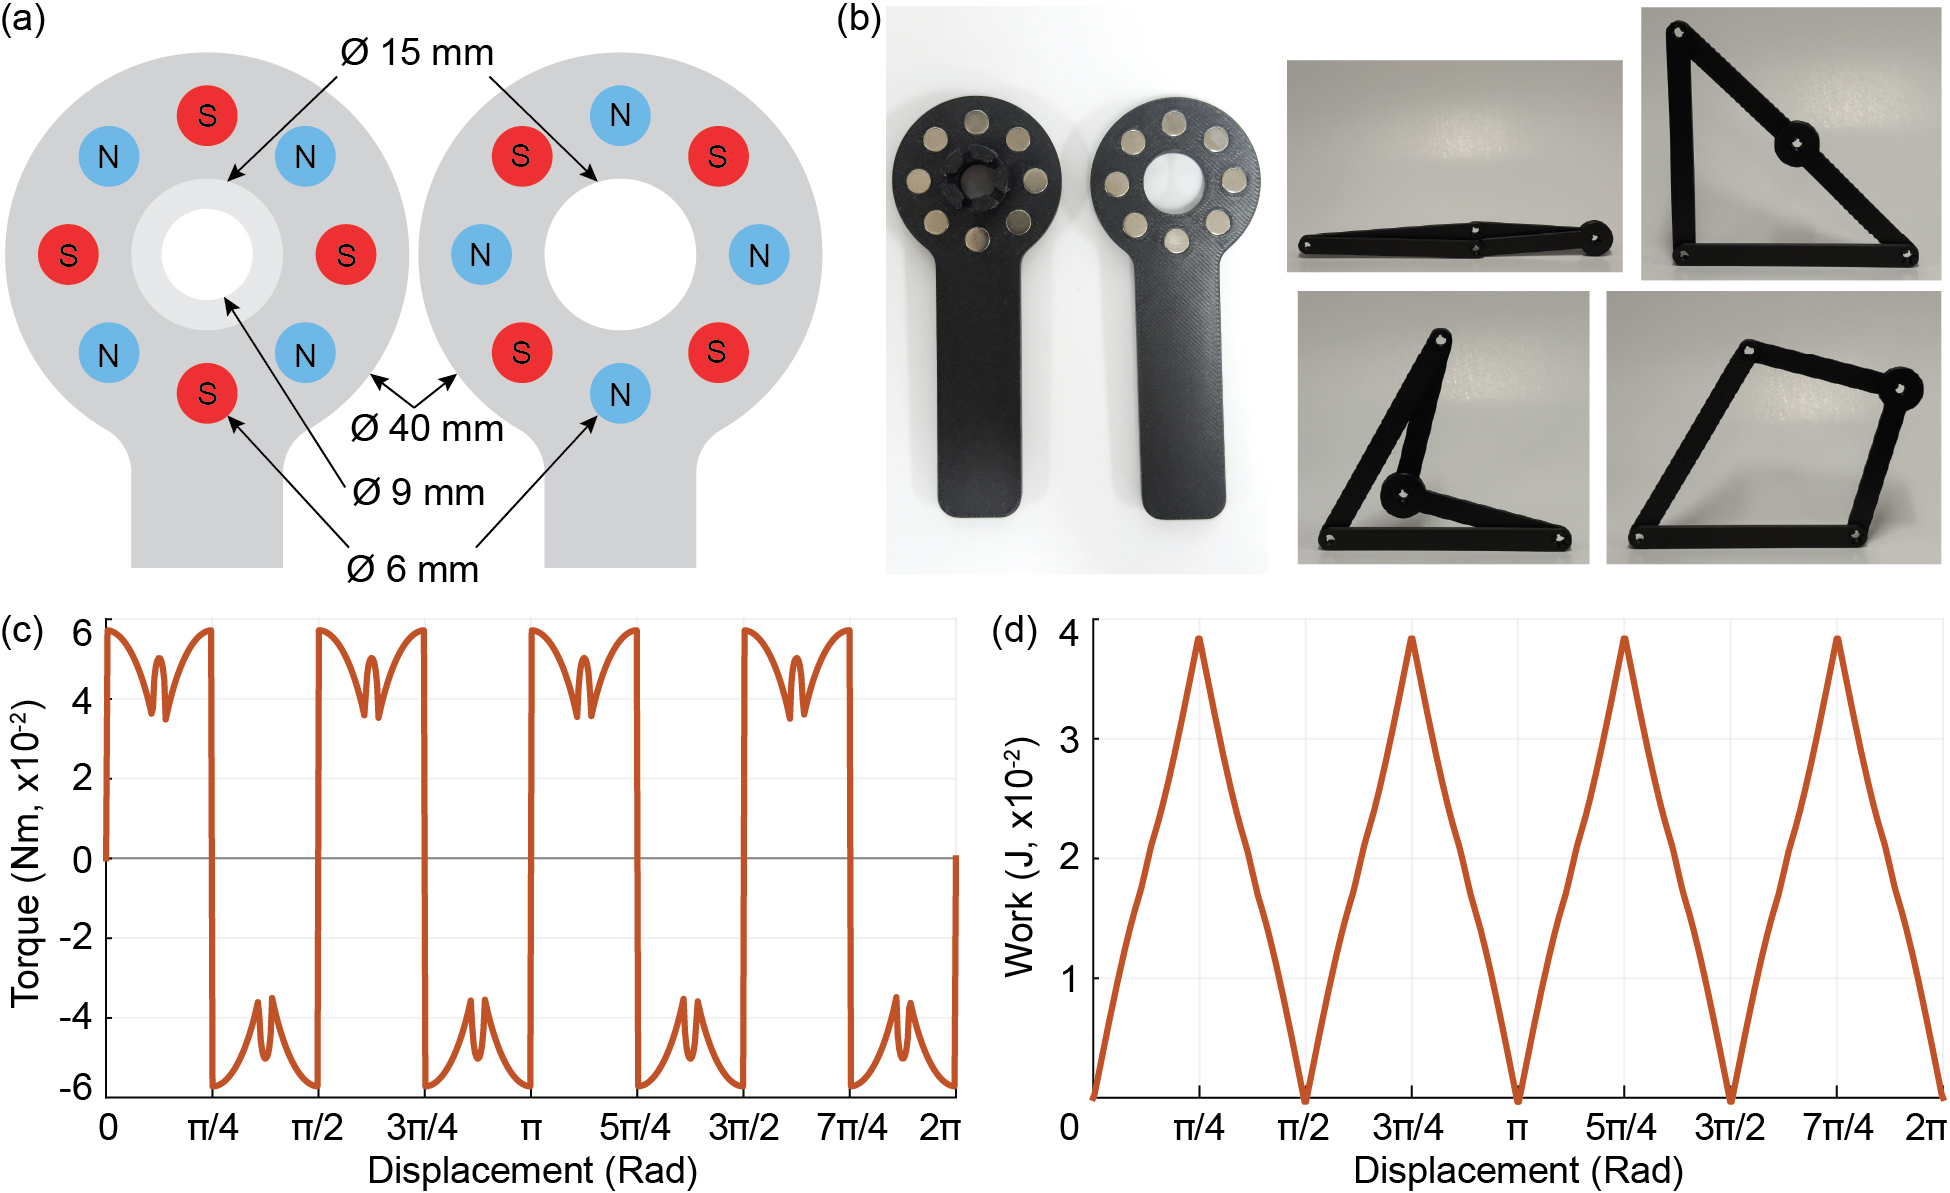
\includegraphics[width=\textwidth]{01-figures/04-03-magnetic-hinge-prototype.jpg}
  \caption{Magnetic multistable torsional hinge prototype: (a) Magnet placement and dimensions of the torsional hinge hub; (b) 3D printed and assembled prototype of a magnetic multistable hinge in a 4-bar linkage unit; Simulated behavior of the magnetic multistable torsional hinge using a reduced-order magnetic interaction model: (c) Torque-displacement, and (d) Work-displacement response over one full rotation.}\label{fig-magnetic-prototype}
\end{figure}

A reduced-order magnetic interaction model is used to estimate the torque required to drive the hinge through multiple stable states and the corresponding work associated with this rotation. The model provides a simple way to interpret the periodic peaks and troughs in the energy landscape produced by the alternating magnet-polarity pattern. The resulting torque-displacement and work–displacement relationships are later used to model multistable hinge behavior in the 3NTS element for multistable reconfigurable truss simulations.

Each magnet is modeled as a cylindrical disc with diameter \(D\), radius \(r=D/2\), thickness \(t\), remanence \(B_r\), and axial gap \(g\) between the magnets. The axial magnetic field at the opposing face is approximated as:
\begin{equation}
B =\frac{B_r}{2}\left[\frac{z_1}{\sqrt{z_1^2+r^2}}-\frac{z_0} {\sqrt{z_0^2+r^2}}\right]
\end{equation}
where, \(z_0 = g\) and \(z_1 = g + t\). The corresponding magnetic pressure is estimated using
\begin{equation}
P = \frac{B^2}{2\mu_0}
\end{equation}
where \(\mu_0 = 4\pi \times 10^{-7}\ \mathrm{N/A^2}\) is the permeability of the free space. The units of \(P\) are N/m\(^2\), which are equivalent to J/m\(^3\). Therefore, the magnetic pressure can be interpreted as an approximate magnetic energy density. In this reduced-order model, the magnetic energy is estimated by multiplying this energy density by the effective interaction volume between the magnets. The force associated with a change in magnet position is then obtained by differentiating the magnetic energy with respect to the corresponding displacement direction.

For the rotating assembly, one hub face is held fixed while the opposing hub face rotates over it. The effective overlap area between the two magnet arrays is denoted by \(A(\theta)\), where \(\theta\) is the angular position of the rotating face of the hub. The total magnetic interaction energy of the system at any given instance then becomes
\begin{equation}
U(\theta) \approx PV(\theta)
\end{equation}
where \(V(\theta)=\ell A(\theta)\) is the effective interaction volume between the two hub faces and \(\ell=t+g\) is the interaction height, taken as the sum of the magnet thickness and axial gap. The torque associated with the magnetic interaction is approximated from the rate of change of the overlap area with respect to the angular displacement  \(\theta\):
\begin{equation}
\tau(\theta) \approx - P \ell \frac{dA}{d\theta}
\end{equation}

The simulated torque required to rotate the magnetic multistable hinge and the corresponding work are shown in Fig.~\ref{fig-magnetic-prototype}\,(c) and (d), respectively. The alternating magnet polarity produces a periodic response with a period of \(\pi/2\) radians, resulting in four repeating regions over one full rotation. In the torque-rotation response, sharp transitions occur from a positive to negative torque as magnet pairs on either face switch between attractive and repulsive configurations. The corresponding work-rotation response forms a periodic energy landscape with four repeated energy wells. The local minima correspond to stable configurations, while the local maxima represent energy barriers between adjacent stable states. These four energy minima are consistent with the stable states observed in the fabricated four-bar linkage prototype.

\subsection{Computational Modeling of Multistable Magnetic Torsional Hinge for Matrix Structural Analysis}\label{04-subsec-magnetic-hinge-model}
\begin{figure}[!ht]
  \centering
  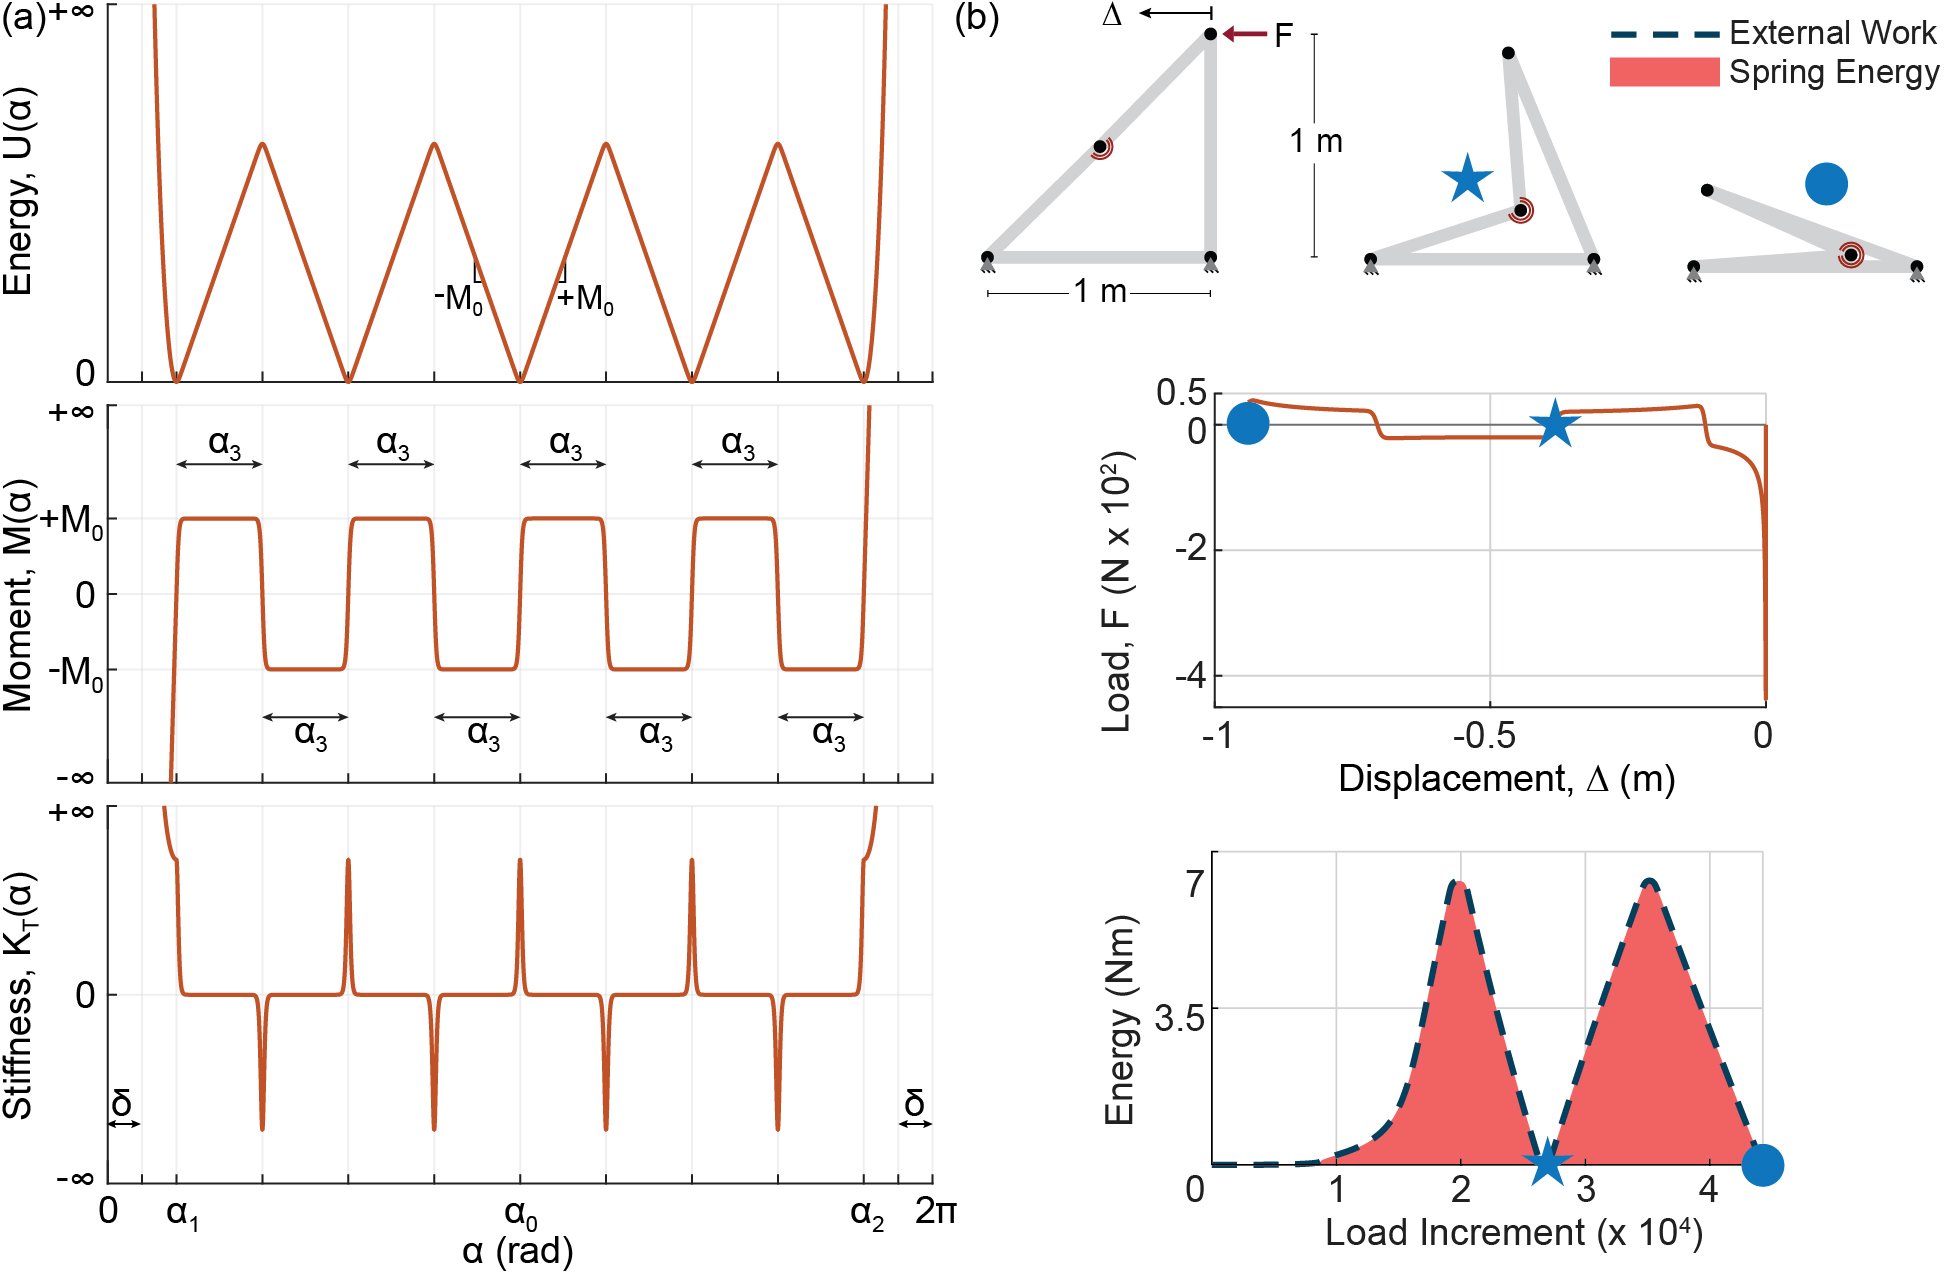
\includegraphics[width=\textwidth]{01-figures/04-04-magnetic-hinge-modeling.jpg}
  \caption{Bistable torsional hinge: (a) Schematic representation of the strain energy (top), restoring moment (middle), and tangent stiffness (bottom) curves for a multistable magnetic torsional hinge with respect to the relative angle of the hinge; (b) Load vs. Displacement (left) and System energy vs. Displacement (right) curves for the buckling of colinear bars in compression fitted with a bistable torsional hinge.}\label{fig-magnetic-hinge}
\end{figure}
Within the central angular interval \(\alpha_1<\alpha<\alpha_2\), the
magnetic multistable hinge is described using the relative rotation
\begin{equation}
\theta=\alpha-\alpha_0,
\label{eq:theta}
\end{equation}
where \(\alpha_0\) is the reference angle. The response outside
\(\alpha_1<\alpha<\alpha_2\) is modeled using the enhanced spring law described
in the preceding section.

The hinge combines a weak linear stiffness with a periodic magnetic
contribution. The two stiffness scales are
\begin{equation}
K_1=\frac{k_0}{10^4},
\qquad
K_2=k_0,
\label{eq:stiffness-scales}
\end{equation}
where \(K_1\) controls the weak background stiffness and \(K_2\) controls the
magnitude of the magnetic contribution. Let \(N=n_{\mathrm{peaks}}\) denote the
number of magnetic periods on each side of \(\theta=0\). The period is
\begin{equation}
p=\frac{\alpha_2-\alpha_0}{N},
\label{eq:period}
\end{equation}
so that, for the symmetric central region,
\begin{equation}
\alpha_1=\alpha_0-Np,
\qquad
\alpha_2=\alpha_0+Np.
\label{eq:symmetric-central-region}
\end{equation}

The smoothing width is
\begin{equation}
\varepsilon=\frac{\pi}{180}\,\varepsilon_{\mathrm{deg}},
\label{eq:smoothing-width}
\end{equation}
where \(\varepsilon_{\mathrm{deg}}\) is specified in degrees. Smaller
\(\varepsilon\) produces sharper magnetic transitions, while larger
\(\varepsilon\) produces smoother transitions.

For each magnetic period, define the local phase coordinate
\(\varphi\in[0,p]\). The three smooth transition functions within a period are
centered at \(\varphi=0\), \(\varphi=p/2\), and \(\varphi=p\). Define
\begin{align}
\mathcal{T}(\varphi)
&=
\tanh\!\left(\frac{\varphi}{\varepsilon}\right)
-\tanh\!\left(\frac{\varphi-\frac{p}{2}}{\varepsilon}\right)
+\tanh\!\left(\frac{\varphi-p}{\varepsilon}\right),
\label{eq:T-shape}\\
\mathcal{S}(\varphi)
&=
\operatorname{sech}^2\!\left(\frac{\varphi}{\varepsilon}\right)
-\operatorname{sech}^2\!\left(\frac{\varphi-\frac{p}{2}}{\varepsilon}\right)
+\operatorname{sech}^2\!\left(\frac{\varphi-p}{\varepsilon}\right).
\label{eq:S-shape}
\end{align}
Here \(\mathcal{T}\) defines the smooth magnetic moment shape within one
period, and \(\mathcal{S}=d\mathcal{T}/d(\varphi/\varepsilon)\) defines the
corresponding stiffness shape.

The energy primitive uses
\begin{equation}
\operatorname{logCosh}(x)
=
|x|+\log\!\left(1+\exp[-2|x|]\right)-\log 2,
\label{eq:logcosh}
\end{equation}
with the constant
\begin{equation}
c_0=
\operatorname{logCosh}(0)
-\operatorname{logCosh}\!\left(-\frac{p}{2\varepsilon}\right)
+\operatorname{logCosh}\!\left(-\frac{p}{\varepsilon}\right).
\label{eq:c0}
\end{equation}
The corresponding dimensionless energy shape is
\begin{equation}
\mathcal{E}(\varphi)
=
\operatorname{logCosh}\!\left(\frac{\varphi}{\varepsilon}\right)
-\operatorname{logCosh}\!\left(\frac{\varphi-\frac{p}{2}}{\varepsilon}\right)
+\operatorname{logCosh}\!\left(\frac{\varphi-p}{\varepsilon}\right)
-c_0.
\label{eq:E-shape}
\end{equation}

For the \(m\)-th magnetic period, where \(m=0,1,\ldots,N-1\), the local phase
coordinate is
\begin{equation}
\varphi_m^+(\theta)=\theta-mp,
\qquad
mp<\theta\le(m+1)p,
\label{eq:positive-phase}
\end{equation}
on the positive side, and
\begin{equation}
\varphi_m^-(\theta)=-\theta-mp,
\qquad
-(m+1)p\le\theta< -mp,
\label{eq:negative-phase}
\end{equation}
on the negative side.

The restoring moment in the central region can then be written as the case
equation
\begin{equation}
M(\theta)=
\begin{cases}
K_1\theta
-K_2\mathcal{T}\!\left(\varphi_m^-(\theta)\right),
& -(m+1)p\le\theta< -mp,\\[8pt]
0,
& \theta=0,\\[8pt]
K_1\theta
+K_2\mathcal{T}\!\left(\varphi_m^+(\theta)\right),
& mp<\theta\le(m+1)p,
\end{cases}
\qquad m=0,1,\ldots,N-1.
\label{eq:moment-cases}
\end{equation}

The tangent stiffness is
\begin{equation}
k_T(\theta)=
\begin{cases}
K_1+\dfrac{K_2}{\varepsilon}
\mathcal{S}\!\left(\varphi_m^-(\theta)\right),
& -(m+1)p\le\theta< -mp,\\[12pt]
K_1+\dfrac{K_2}{\varepsilon}\mathcal{S}(0),
& \theta=0,\\[12pt]
K_1+\dfrac{K_2}{\varepsilon}
\mathcal{S}\!\left(\varphi_m^+(\theta)\right),
& mp<\theta\le(m+1)p,
\end{cases}
\qquad m=0,1,\ldots,N-1.
\label{eq:stiffness-cases}
\end{equation}

Finally, the strain energy is
\begin{equation}
U(\theta)=
\begin{cases}
\dfrac{1}{2}K_1\theta^2
+K_2\varepsilon\,\mathcal{E}\!\left(\varphi_m^-(\theta)\right),
& -(m+1)p\le\theta< -mp,\\[12pt]
0,
& \theta=0,\\[8pt]
\dfrac{1}{2}K_1\theta^2
+K_2\varepsilon\,\mathcal{E}\!\left(\varphi_m^+(\theta)\right),
& mp<\theta\le(m+1)p,
\end{cases}
\qquad m=0,1,\ldots,N-1.
\label{eq:energy-cases}
\end{equation}
Equations~\eqref{eq:moment-cases}--\eqref{eq:energy-cases} define the magnetic
multistable hinge law used for \(\alpha_1<\alpha<\alpha_2\).


\section{Bi-Stable Torsional Springs}\label{04-sec-bistable-spring}
The piecewise torsional spring formulation introduced in the previous section provides a controlled way to restrict hinge rotation within a prescribed angular range. The next step is to extend this idea to hinges with nonlinear rotational response. Such hinges are useful when the structure is intended to store and release energy through large rotations, or when the hinge must exhibit multiple stable configurations.

A common way to formulate the mechanical response of a structural element is to begin with a strain energy function. The internal force is obtained by differentiating the strain energy with respect to the deformation variable, and the tangent stiffness is obtained by differentiating the internal force. For a rotational spring, this means that the restoring moment is derived from the strain energy with respect to the hinge angle, and the tangent stiffness is derived from the restoring moment. This approach is convenient when the strain energy function is smooth and differentiable over the full deformation range.

This requirement becomes more restrictive when the hinge response is nonlinear and piecewise-defined. In such cases, continuity must be enforced at every transition point between adjacent branches. The strain energy, restoring moment, and tangent stiffness should remain compatible across these points to avoid artificial jumps in the mechanical response. These jumps are especially problematic in nonlinear equilibrium solvers, such as arc-length or generalized displacement-control methods, because the solver relies on a consistent tangent stiffness to trace the equilibrium path.

The difficulty becomes greater when the hinge is designed to be bistable. Bistability requires the strain energy to have two local minima separated by an energy barrier. This produces a nonlinear moment–rotation response with regions of positive and negative tangent stiffness. Although such behavior can be represented using high-order polynomials or trigonometric functions, constructing a piecewise strain energy function that satisfies all boundary conditions, preserves smoothness after differentiation, and produces the intended stable equilibria is not straightforward.

For this reason, the bistable hinge response is formulated here by prescribing the restoring moment directly rather than by first defining the strain energy. The restoring moment is chosen as a smooth function of the hinge angle, and the tangent stiffness is then obtained by differentiating this moment with respect to rotation. The corresponding strain energy can still be recovered by integrating the restoring moment over the hinge rotation. This approach provides more direct control over the engineered rotational response while preserving a mechanically consistent energy interpretation.

Using this formulation, the bistable torsional spring is defined through the following restoring moment and tangent stiffness functions.
\begin{figure}[!ht]
  \centering
  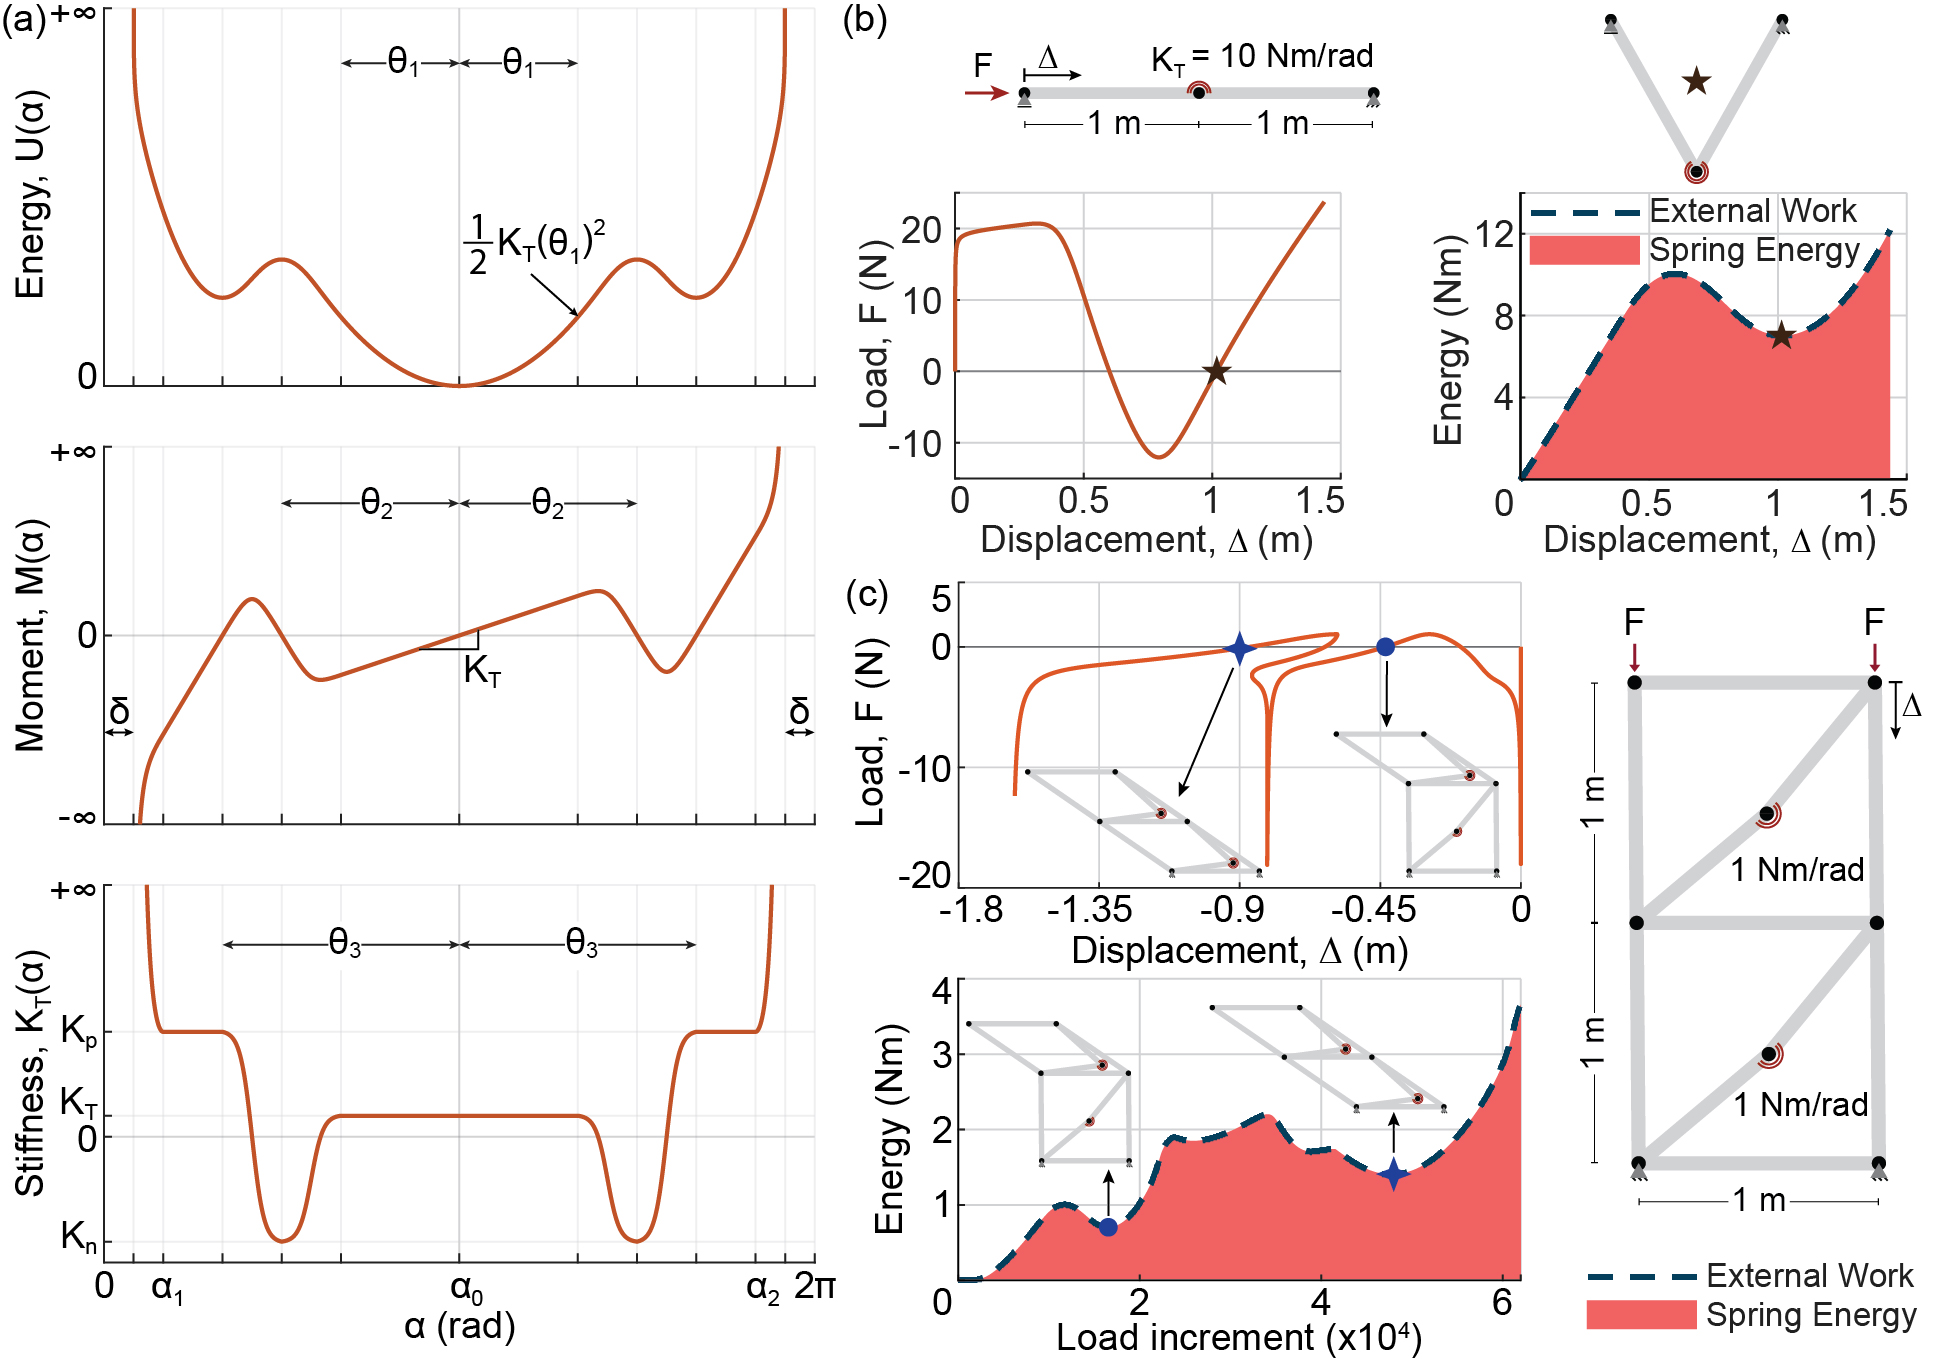
\includegraphics[width=\textwidth]{01-figures/04-05-bistable-hinge-modeling.jpg}
  \caption{Bistable torsional hinge: (a) Schematic representation of the strain energy (top), restoring moment (middle), and tangent stiffness (bottom) curves for a bistable torsional hinge with respect to the relative angle of the hinge; (b) Load vs. Displacement (left) and System energy vs. Displacement (right) curves for the buckling of colinear bars in compression fitted with a bistable torsional hinge.}\label{fig-bistable-hinge}
\end{figure}
\subsection{Computational Formulation of Bistable Torsional Spring for Matrix Structural Analysis}\label{04-subsec-bistable-equations}
Within the central angular interval \(\alpha_1<\alpha<\alpha_2\), the
bistable torsional spring is described using the relative rotation
\begin{equation}
\theta=\alpha-\alpha_0,
\label{eq:theta}
\end{equation}
where \(\alpha_0\) is the stress-free reference angle. The response outside
\(\alpha_1<\alpha<\alpha_2\) is modeled using the enhanced spring law described
in the preceding section.

The spring is defined by an initial stiffness \(K_T\), a negative stiffness
\(k_{\mathrm{neg}}\), and a post-transition positive stiffness
\(k_{\mathrm{pos}}\). The transition rotations satisfy
\begin{equation}
0<\theta_1<\theta_2<\theta_3.
\label{eq:transition-widths}
\end{equation}
The smooth transition function is
\begin{equation}
q(s)=
\frac{
\tanh\!\left[\beta\left(s-\frac{1}{2}\right)\right]
+\tanh\!\left(\frac{\beta}{2}\right)
}{
2\tanh\!\left(\frac{\beta}{2}\right)
},
\qquad 0\le s\le 1,
\label{eq:q}
\end{equation}
where \(s\) is the local normalized coordinate within a transition interval and
\(\beta\) controls the sharpness of the transition. The function satisfies
\(q(0)=0\) and \(q(1)=1\), so it smoothly interpolates between two prescribed
stiffness values over one transition interval. Larger values of \(\beta\)
produce a sharper transition, while smaller values produce a more gradual
transition. Its first and second primitives are denoted by
\begin{equation}
Q(s)=\int_0^s q(u)\,du,
\qquad
\mathcal{Q}(s)=\int_0^s Q(v)\,dv.
\label{eq:q-primitives}
\end{equation}

The moment levels at the positive transition rotations are
\begin{align}
M_1 &= K_T\theta_1, \label{eq:M1}\\
M_2 &=
M_1
+(\theta_2-\theta_1)
\left[
K_T+\left(k_{\mathrm{neg}}-K_T\right)Q(1)
\right],
\label{eq:M2}\\
M_3 &=
M_2
+(\theta_3-\theta_2)
\left[
k_{\mathrm{neg}}
+\left(k_{\mathrm{pos}}-k_{\mathrm{neg}}\right)Q(1)
\right].
\label{eq:M3}
\end{align}
The corresponding energy levels are
\begin{align}
U_1 &=
\frac{1}{2}K_T\theta_1^2, \label{eq:U1}\\
U_2 &=
U_1+(\theta_2-\theta_1)M_1
+(\theta_2-\theta_1)^2
\left[
\frac{1}{2}K_T
+\left(k_{\mathrm{neg}}-K_T\right)\mathcal{Q}(1)
\right],
\label{eq:U2}\\
U_3 &=
U_2+(\theta_3-\theta_2)M_2
+(\theta_3-\theta_2)^2
\left[
\frac{1}{2}k_{\mathrm{neg}}
+\left(k_{\mathrm{pos}}-k_{\mathrm{neg}}\right)\mathcal{Q}(1)
\right].
\label{eq:U3}
\end{align}

The tangent stiffness in the central region is
\begin{equation}
k_T(\theta)=
\begin{cases}
k_{\mathrm{pos}},
& \theta<-\theta_3,\\[4pt]
k_{\mathrm{neg}}
+\left(k_{\mathrm{pos}}-k_{\mathrm{neg}}\right)
q\!\left(\dfrac{-\theta-\theta_2}{\theta_3-\theta_2}\right),
& -\theta_3\le\theta<-\theta_2,\\[12pt]
K_T+\left(k_{\mathrm{neg}}-K_T\right)
q\!\left(\dfrac{-\theta-\theta_1}{\theta_2-\theta_1}\right),
& -\theta_2\le\theta<-\theta_1,\\[12pt]
K_T,
& -\theta_1\le\theta\le\theta_1,\\[4pt]
K_T+\left(k_{\mathrm{neg}}-K_T\right)
q\!\left(\dfrac{\theta-\theta_1}{\theta_2-\theta_1}\right),
& \theta_1<\theta\le\theta_2,\\[12pt]
k_{\mathrm{neg}}
+\left(k_{\mathrm{pos}}-k_{\mathrm{neg}}\right)
q\!\left(\dfrac{\theta-\theta_2}{\theta_3-\theta_2}\right),
& \theta_2<\theta\le\theta_3,\\[12pt]
k_{\mathrm{pos}},
& \theta>\theta_3.
\end{cases}
\label{eq:stiffness}
\end{equation}

The restoring moment is obtained by integrating the stiffness with respect to
\(\theta\) and enforcing \(M(0)=0\):
\begin{equation}
M(\theta)=
\begin{cases}
-M_3+k_{\mathrm{pos}}(\theta+\theta_3),
& \theta<-\theta_3,\\[6pt]
-M_2-(\theta_3-\theta_2)\left[
k_{\mathrm{neg}}s_+^-
+\left(k_{\mathrm{pos}}-k_{\mathrm{neg}}\right)Q(s_+^-)
\right],
& -\theta_3\le\theta<-\theta_2,\\[10pt]
-M_1-(\theta_2-\theta_1)\left[
K_Ts_-^-
+\left(k_{\mathrm{neg}}-K_T\right)Q(s_-^-)
\right],
& -\theta_2\le\theta<-\theta_1,\\[10pt]
K_T\theta,
& -\theta_1\le\theta\le\theta_1,\\[6pt]
M_1+(\theta_2-\theta_1)\left[
K_Ts_-^+
+\left(k_{\mathrm{neg}}-K_T\right)Q(s_-^+)
\right],
& \theta_1<\theta\le\theta_2,\\[10pt]
M_2+(\theta_3-\theta_2)\left[
k_{\mathrm{neg}}s_+^+
+\left(k_{\mathrm{pos}}-k_{\mathrm{neg}}\right)Q(s_+^+)
\right],
& \theta_2<\theta\le\theta_3,\\[10pt]
M_3+k_{\mathrm{pos}}(\theta-\theta_3),
& \theta>\theta_3,
\end{cases}
\label{eq:moment}
\end{equation}
where the scaled transition coordinates are
\begin{equation}
s_-^-=\frac{-\theta-\theta_1}{\theta_2-\theta_1},
\qquad
s_+^-=\frac{-\theta-\theta_2}{\theta_3-\theta_2},
\qquad
s_-^+=\frac{\theta-\theta_1}{\theta_2-\theta_1},
\qquad
s_+^+=\frac{\theta-\theta_2}{\theta_3-\theta_2}.
\label{eq:s-coordinates}
\end{equation}

The strain energy is defined by \(U(0)=0\) and
\(M=dU/d\theta\). In the central region,
\begin{equation}
U(\theta)=
\begin{cases}
U_3-M_3(\theta+\theta_3)
+\dfrac{1}{2}k_{\mathrm{pos}}(\theta+\theta_3)^2,
& \theta<-\theta_3,\\[10pt]
U_2+(\theta_3-\theta_2)M_2s_+^-
+(\theta_3-\theta_2)^2\left[
\dfrac{1}{2}k_{\mathrm{neg}}(s_+^-)^2
+\left(k_{\mathrm{pos}}-k_{\mathrm{neg}}\right)\mathcal{Q}(s_+^-)
\right],
& -\theta_3\le\theta<-\theta_2,\\[14pt]
U_1+(\theta_2-\theta_1)M_1s_-^-
+(\theta_2-\theta_1)^2\left[
\dfrac{1}{2}K_T(s_-^-)^2
+\left(k_{\mathrm{neg}}-K_T\right)\mathcal{Q}(s_-^-)
\right],
& -\theta_2\le\theta<-\theta_1,\\[14pt]
\dfrac{1}{2}K_T\theta^2,
& -\theta_1\le\theta\le\theta_1,\\[10pt]
U_1+(\theta_2-\theta_1)M_1s_-^+
+(\theta_2-\theta_1)^2\left[
\dfrac{1}{2}K_T(s_-^+)^2
+\left(k_{\mathrm{neg}}-K_T\right)\mathcal{Q}(s_-^+)
\right],
& \theta_1<\theta\le\theta_2,\\[14pt]
U_2+(\theta_3-\theta_2)M_2s_+^+
+(\theta_3-\theta_2)^2\left[
\dfrac{1}{2}k_{\mathrm{neg}}(s_+^+)^2
+\left(k_{\mathrm{pos}}-k_{\mathrm{neg}}\right)\mathcal{Q}(s_+^+)
\right],
& \theta_2<\theta\le\theta_3,\\[14pt]
U_3+M_3(\theta-\theta_3)
+\dfrac{1}{2}k_{\mathrm{pos}}(\theta-\theta_3)^2,
& \theta>\theta_3.
\end{cases}
\label{eq:energy}
\end{equation}
Equations~\eqref{eq:stiffness}--\eqref{eq:energy} define the bistable spring
law used for \(\alpha_1<\alpha<\alpha_2\).

\subsection{Structural Response of Reconfigurable Trusses with Bistable Torsional Hinges}\label{04-subsec-bistable-examples}
This subsection presents two example structures fitted with bistable torsional hinges. The examples demonstrate how the proposed formulation can represent highly nonlinear hinge response within the structural analysis of reconfigurable trusses. A physical prototype of this idealized bistable torsional spring has not yet been developed. Therefore, the examples are intended as computational demonstrations of the modeling capability. They show how bistable hinge laws can be used to study snap-through, post-transition stiffening, and transitions between multiple stable states.

Both examples use the bistable torsional spring law described in the previous subsection. The bistable hinge's transition points are set to \(\theta_1=60^\circ{}\), \(\theta_2=90^\circ{}\), and \(\theta_3=120^\circ{}\). The negative stiffness value is defined using \(K_n=-5K_T\), and the post-transition positive stiffness branch is defined using \(K_p=5K_T\). The admissible hinge rotation is bounded using the same asymptotic stiffening strategy introduced in the enhanced spring law from Section~\ref{04-subsec-enhanced-spring}. The corresponding angular-limit parameters are \(\delta=15^\circ{}\), \(\alpha_1=30^\circ{}\), and \(\alpha_2=330^\circ{}\). These limits restrict the deformation of the hinge in the inverval (15\(^\circ\), 345\(^\circ\)).

The first example consists of two collinear bars connected by a bistable torsional hinge and loaded in compression, as shown in Fig.~\ref{fig-bistable-hinge},(b). The left end is modeled as a roller support, the right end is modeled as a pinned support, and the bistable torsional spring is placed at the connection between the two bars. Each bar has a length of 1~m, elastic modulus \(E=3\times10^9~\text{N/m}^2\), and cross-sectional area \(A=0.5~\text{m}^2\). The baseline torsional spring stiffness is \(K_T=10~\text{Nm/rad}\).

As the imposed displacement (\Delta) increases in the positive (x)-direction, the applied load initially rises to approximately 20~N. An elastic instability then develops at the central hinge, and the structure snaps away from the initial collinear configuration. During this transition, the load required to continue deformation decreases and becomes negative. This response indicates that the structure tends to move toward the next stable state once the instability is triggered. The second stable state occurs near \(\Delta=1~\text{m}\). This configuration is marked with a star on the load-displacement curve, the energy plot, and the corresponding deformed configuration in Fig.~\ref{fig-bistable-hinge},(b). At this state, the spring-energy curve exhibits a local minimum, which is consistent with a stable equilibrium configuration. Further displacement beyond this point drives the hinge into the post-transition positive-stiffness regime. As a result, the applied load increases again.

The second example considers a reconfigurable truss with two independent kinematic degrees of freedom. The structure, shown in Fig.~\ref{fig-bistable-hinge}\,(c), is the same stacked square-linkage truss introduced in Fig.~\ref{fig-deployment-path}\,(a), but each spring is now modeled as a bistable torsional hinge. In this example, the baseline torsional stiffness is set to \(K_T=1~\text{Nm/rad}\) for each hinge.

As vertical compression is applied to the structure, the load magnitude first increases rapidly with little global displacement. An elastic instability then develops in the upper square-linkage unit. The upper unit snaps into its next stable state, producing a sharp drop in the applied load. This first stable state is marked with a blue circle in Fig.~\ref{fig-bistable-hinge},(c). After this transition, the upper hinge enters its post-transition positive-stiffness branch, and additional deformation is redirected to the lower unit.

With continued compression, the load rises again until a second instability develops in the lower square-linkage unit. The lower unit then snaps into its next stable state. This second stable state is marked with a blue star in Fig.~\ref{fig-bistable-hinge},(c). The blue circle and blue star are also identified on the spring-energy plot, where they correspond to local minima associated with stable equilibrium configurations.

These examples show that bistable torsional hinges can introduce multiple stable configurations into reconfigurable trusses. In the single-hinge example, the structure transitions between two stable states. In the stacked truss, the two independent kinematic degrees of freedom produce a sequence of stable-state transitions. The analysis therefore demonstrates how nonlinear hinge laws can be used to program the deployment path and stable configurations of reconfigurable truss systems.

\section{Discussion}\label{04-sec-discussion}

\section{Concluding Remarks}\label{04-sec-conclusion}